\documentclass[12pt]{article}

\usepackage[a4paper, margin=1in]{geometry}
\usepackage{graphicx}
\usepackage{enumitem}
\usepackage{amsmath}

\title{OMNeT++ IP Scheduler\\\large{Overview, implementation, and analysis}}
\date{2020\\December}
\author{\\Tomas-Adrian Boboi\\Universitatea Politehnica Timișoara}



\begin{document}
    \maketitle
    \pagebreak
    
    \tableofcontents
    \pagebreak
    
    \section{Initial requirements}
        \subsection*{The simulation model}
        The simulation model consists of the following OMNeT++ modules:
        \begin{enumerate}
            \item{A number of mobile users. In the first stages of the model you can implement two identical users, then you can consider a number of K users, organized as an array of users. Each user generates IP packets according to a certain pattern: e.g. an IP packet at certain (random) time intervals, or a user generates files, a file consisting on a (random) number of IP packets. At the beginning the IP packets can be considered of fixed length, i.e. one IP packet = 1500 bytes. A user has a certain priority. There can be for example 3 or 4 priority levels. For 3 priority levels, they are (in increasing order): LP (low priority), medium priority (MP) and HP (high priority). For 4 levels, they are: non real-time (nrt) low priority and nrt HP, real-time (rt) LP and rt HP.}
            \item{A scheduler. The scheduler is situated in the same Omnet module as the queues. The queues are not per user, but per priority class. This means that the packets arriving from LP user will be stored in the LP queue, the packets from MP and respectively HP users will be stored in the MP and respectively HP queue. The scheduler reads the lengths of the queues and implements a scheduling algorithm that determines which queue will send data. The sending of a packet takes a time equal to its length divided by the line rate (i.e. 1500 bytes / 1 Mega bit per second). The scheduler cannot send another packet during this time interval.}
            \item{A sink. The sink models the destination of the data. When the data (i.e. IP) packets created by an user arrive to the sink module, the sink simply deletes the OMNeT++ messages representing the data packets. Also, the sink is used to collect statistics about the simulation, statistics that can be for each user, for each group of users (e.g. Low, Medium and High priority users) and/or for the entire system. These statistical information can be: the number of data packets that arrive to the sink, the mean, minimum and maximum delay of the data packets, etc.}
        \end{enumerate}
        In the OMNeT directories there is one called "samples", with different simulation models implemented in OMNeT++. From these samples, you can use as a starting point for your model the sources from the "fifo" system.
        
        \subsection*{Basic/minimal requirements}
        Implement the simulation model described above. The scheduling algorithm is not very important in this stage, it can be a simple round robin: each nonempty queue sends a data packet. Or it can be a priority queueing algorithm: a queue is not served until there are non-empty higher priority queues.

        \subsection*{For exam, there are two alternatives to improve the project}
        Implement one of the following scheduling algorithms:
        \begin{itemize}
            \item{Priority queueing (a lower priority queue is served if and only if all higher priority queues are empty)}
            \item{A weighted round robin: an action takes place every time when there are resources available. The winner of the action will be served. The criteria for the action is, firstly, the time elapsed since the user was served last time. Then, we can improve the algorithm by introducing weights (positive numbers >1). The time elapsed since the user was served last time is multiplied with user's weight. Then, a user with a higher weight will be served more often. Compare the performance (i.e. average delay, minimum and maximum delay) of the implemented algorithms.}
        \end{itemize}

    \section{Network structure}
    The network is described by the \verb|IpScheduler.ned| file, which contains the users, which generate the IP packets, the packet handler, which handles the packets received from the users, and the sink, which receives the packets sent from the packet handler.

        \subsection{IpScheduler}
        \verb|IpScheduler| is the main network, where all the sub-components reside.
        \begin{figure}[htbp!]
            \centering
            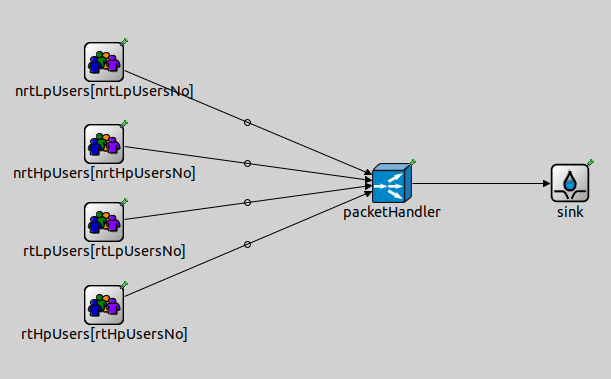
\includegraphics[width=0.8\textwidth]{images/ip_scheduler.png}
            \caption{The main network structure}
        \end{figure}
        \pagebreak
        
        \subsection{PacketHandler}
        \verb|PacketHandler| is the component responsible with receiving the packets from the users, storing them in the corresponding queue, depending on the priority level of the users, scheduling the sending of the packets, and sending the packets to the sink.
        \begin{figure}[htbp!]
            \centering
            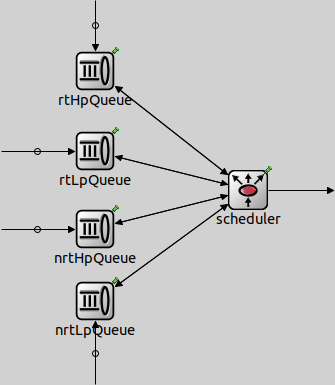
\includegraphics[width=0.45\textwidth]{images/packet_handler.png}
            \caption{The packet handler structure}
        \end{figure}
        
        \subsection{User}
        The \verb|User| is the component which generates IP packets at a certain rate, and sends them to be handled bu the \verb|PacketHandler|. The users are grouped in priority classes:
        \begin{itemize}
            \item{non-real-time, low priority (nrtLp)}
            \item{non-real-time, low priority (nrtHp)}
            \item{real-time, high priority (rtLp)}
            \item{real-time, low priority (rtHp)}
        \end{itemize}
        The size of the generated IP packets, the packet generation rate, and the number of users in each priority class can be configured in the \verb|ipsched/config/users.ini| and \verb|ipsched/config/user_packets.ini| files.

        \subsection{Queue}
        The \verb|Queue| is the module which stores the IP packets generated by the users, and sends them towards the sink, whenever the scheduler allows it. There are four queues, one for each priority class, and they all communicate with the scheduler bidirectionally: they receive control messages from the scheduler, and send packets to the scheduler, when asked to.
        The \textit{Queue} class contains a \verb|cPacketQueue| attribute, where the IP packets are stored.
        The \verb|Queue| module is also responsible with logging each queue's length, so we can collect data about the length of each queue at any given time.
        
        \subsection{Sink}
        The \verb|Sink| is a module whose only purpose is to receive the IP packets, delete them, and record statistics about them (packet lifetime, total number of packets, etc.).

        \subsection{Scheduler}
        The \verb|Scheduler| can be considered the most complex module of the system, and the most important, because it is responsible for deciding which queue sends a packet towards the sink. This job can be accomplished in multiple ways, and the current project provides three scheduler implementations: Priority Queueing, Round Robin, and Weighted Round Robin.

    \section{Scheduler variations}
    The current project provides three implementations for the scheduler, each with its particularities and different levels of efficiency.

        \subsection{Priority Queueing Scheduler}
        \begin{figure}[htbp!]
            \centering
            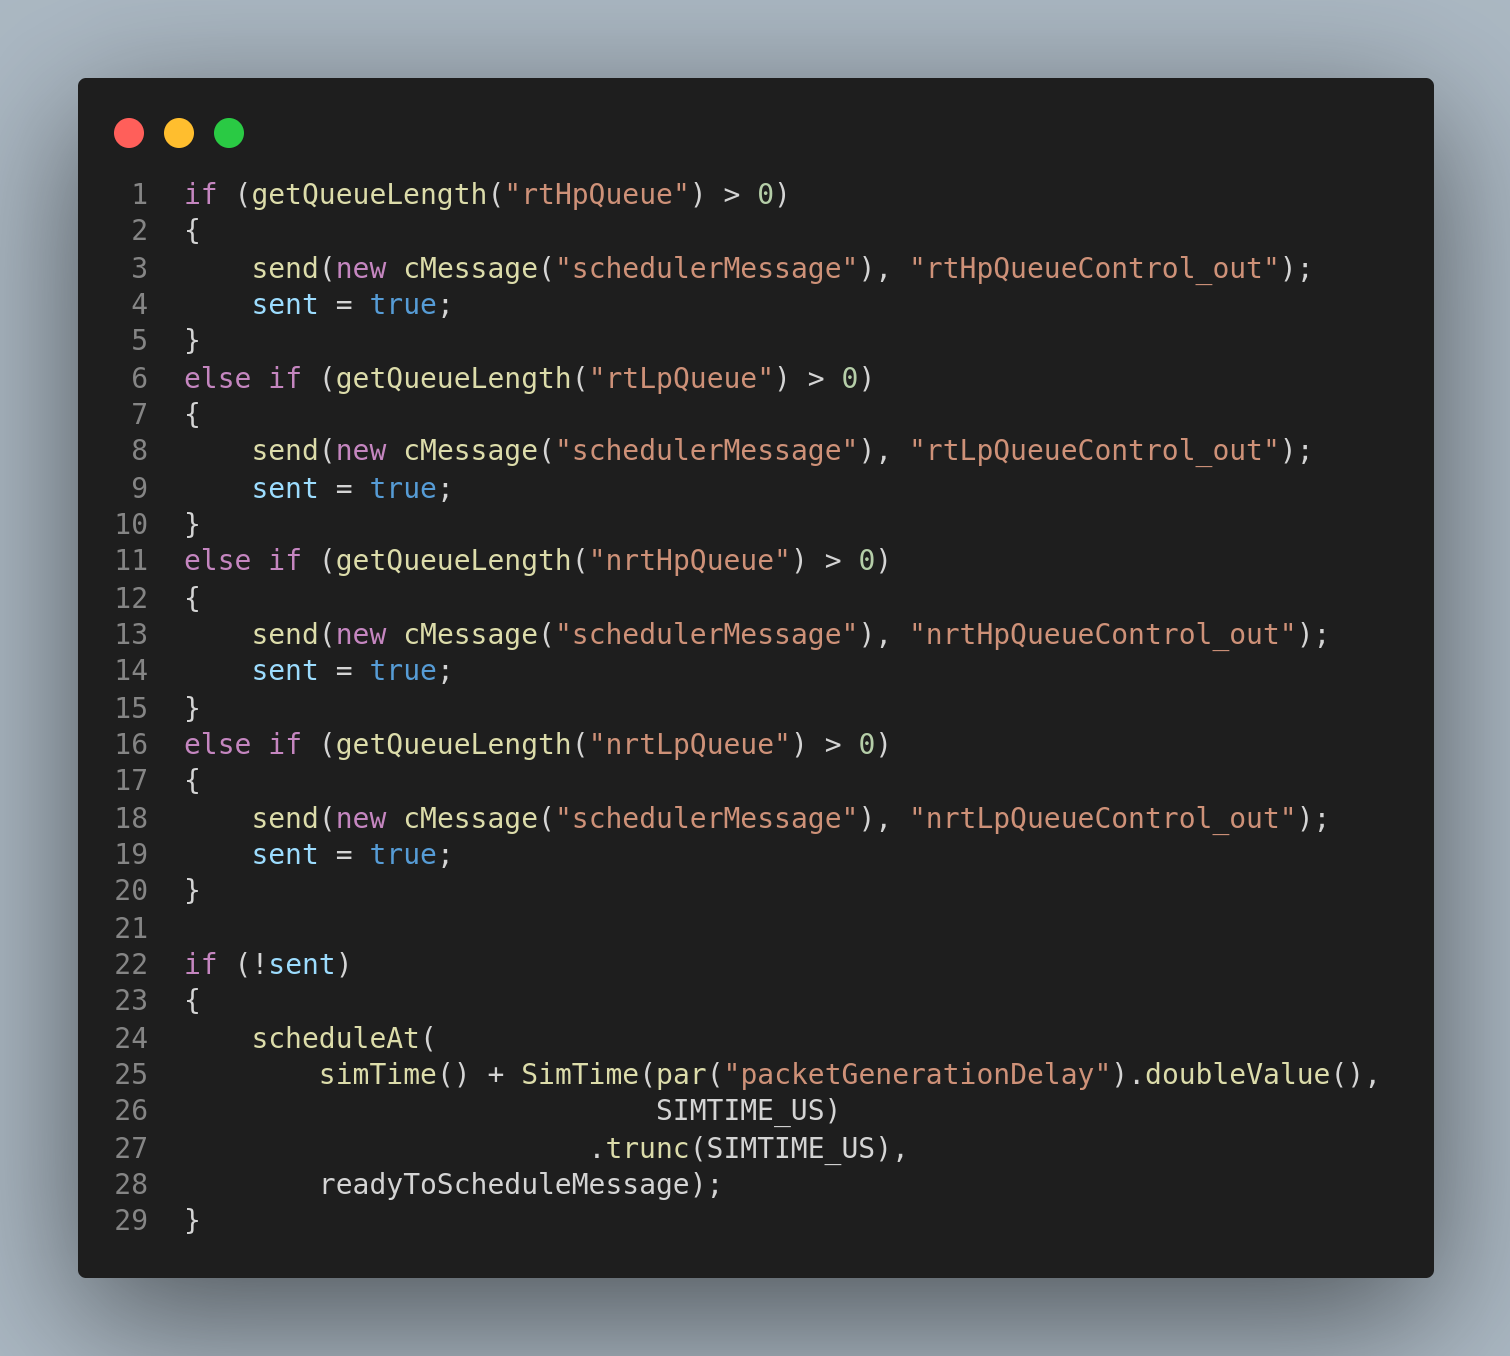
\includegraphics[width=0.9\textwidth]{images/pq_code.png}
            \caption{The inner workings of the Priority Queueing scheduler}
        \end{figure}
        \pagebreak
        The priority queueing algorithm, according to the requirements, allows a queue to send a packet if and only if the higher priority queues are empty.
        
        As we can see in the code, we first check the length of the queue with the highest priority, then, if it is zero, we move on to check the length of the queue below it priority-wise, and so on. If the scheduler decides that a queue should send a packet, it sends a control message to the respective queue, telling it to send a packet. The queue will then receive that message, and know that it came from the scheduler, and sends a packet.
        
        If no packet was requested, that means that all the queues' lengths are zero, and the scheduler enters a sleep state, which is equal to the average time needed for a packet to arrive in any one of the queues.

        \subsection{Round Robin Scheduler}
        \begin{figure}[htbp!]
            \centering
            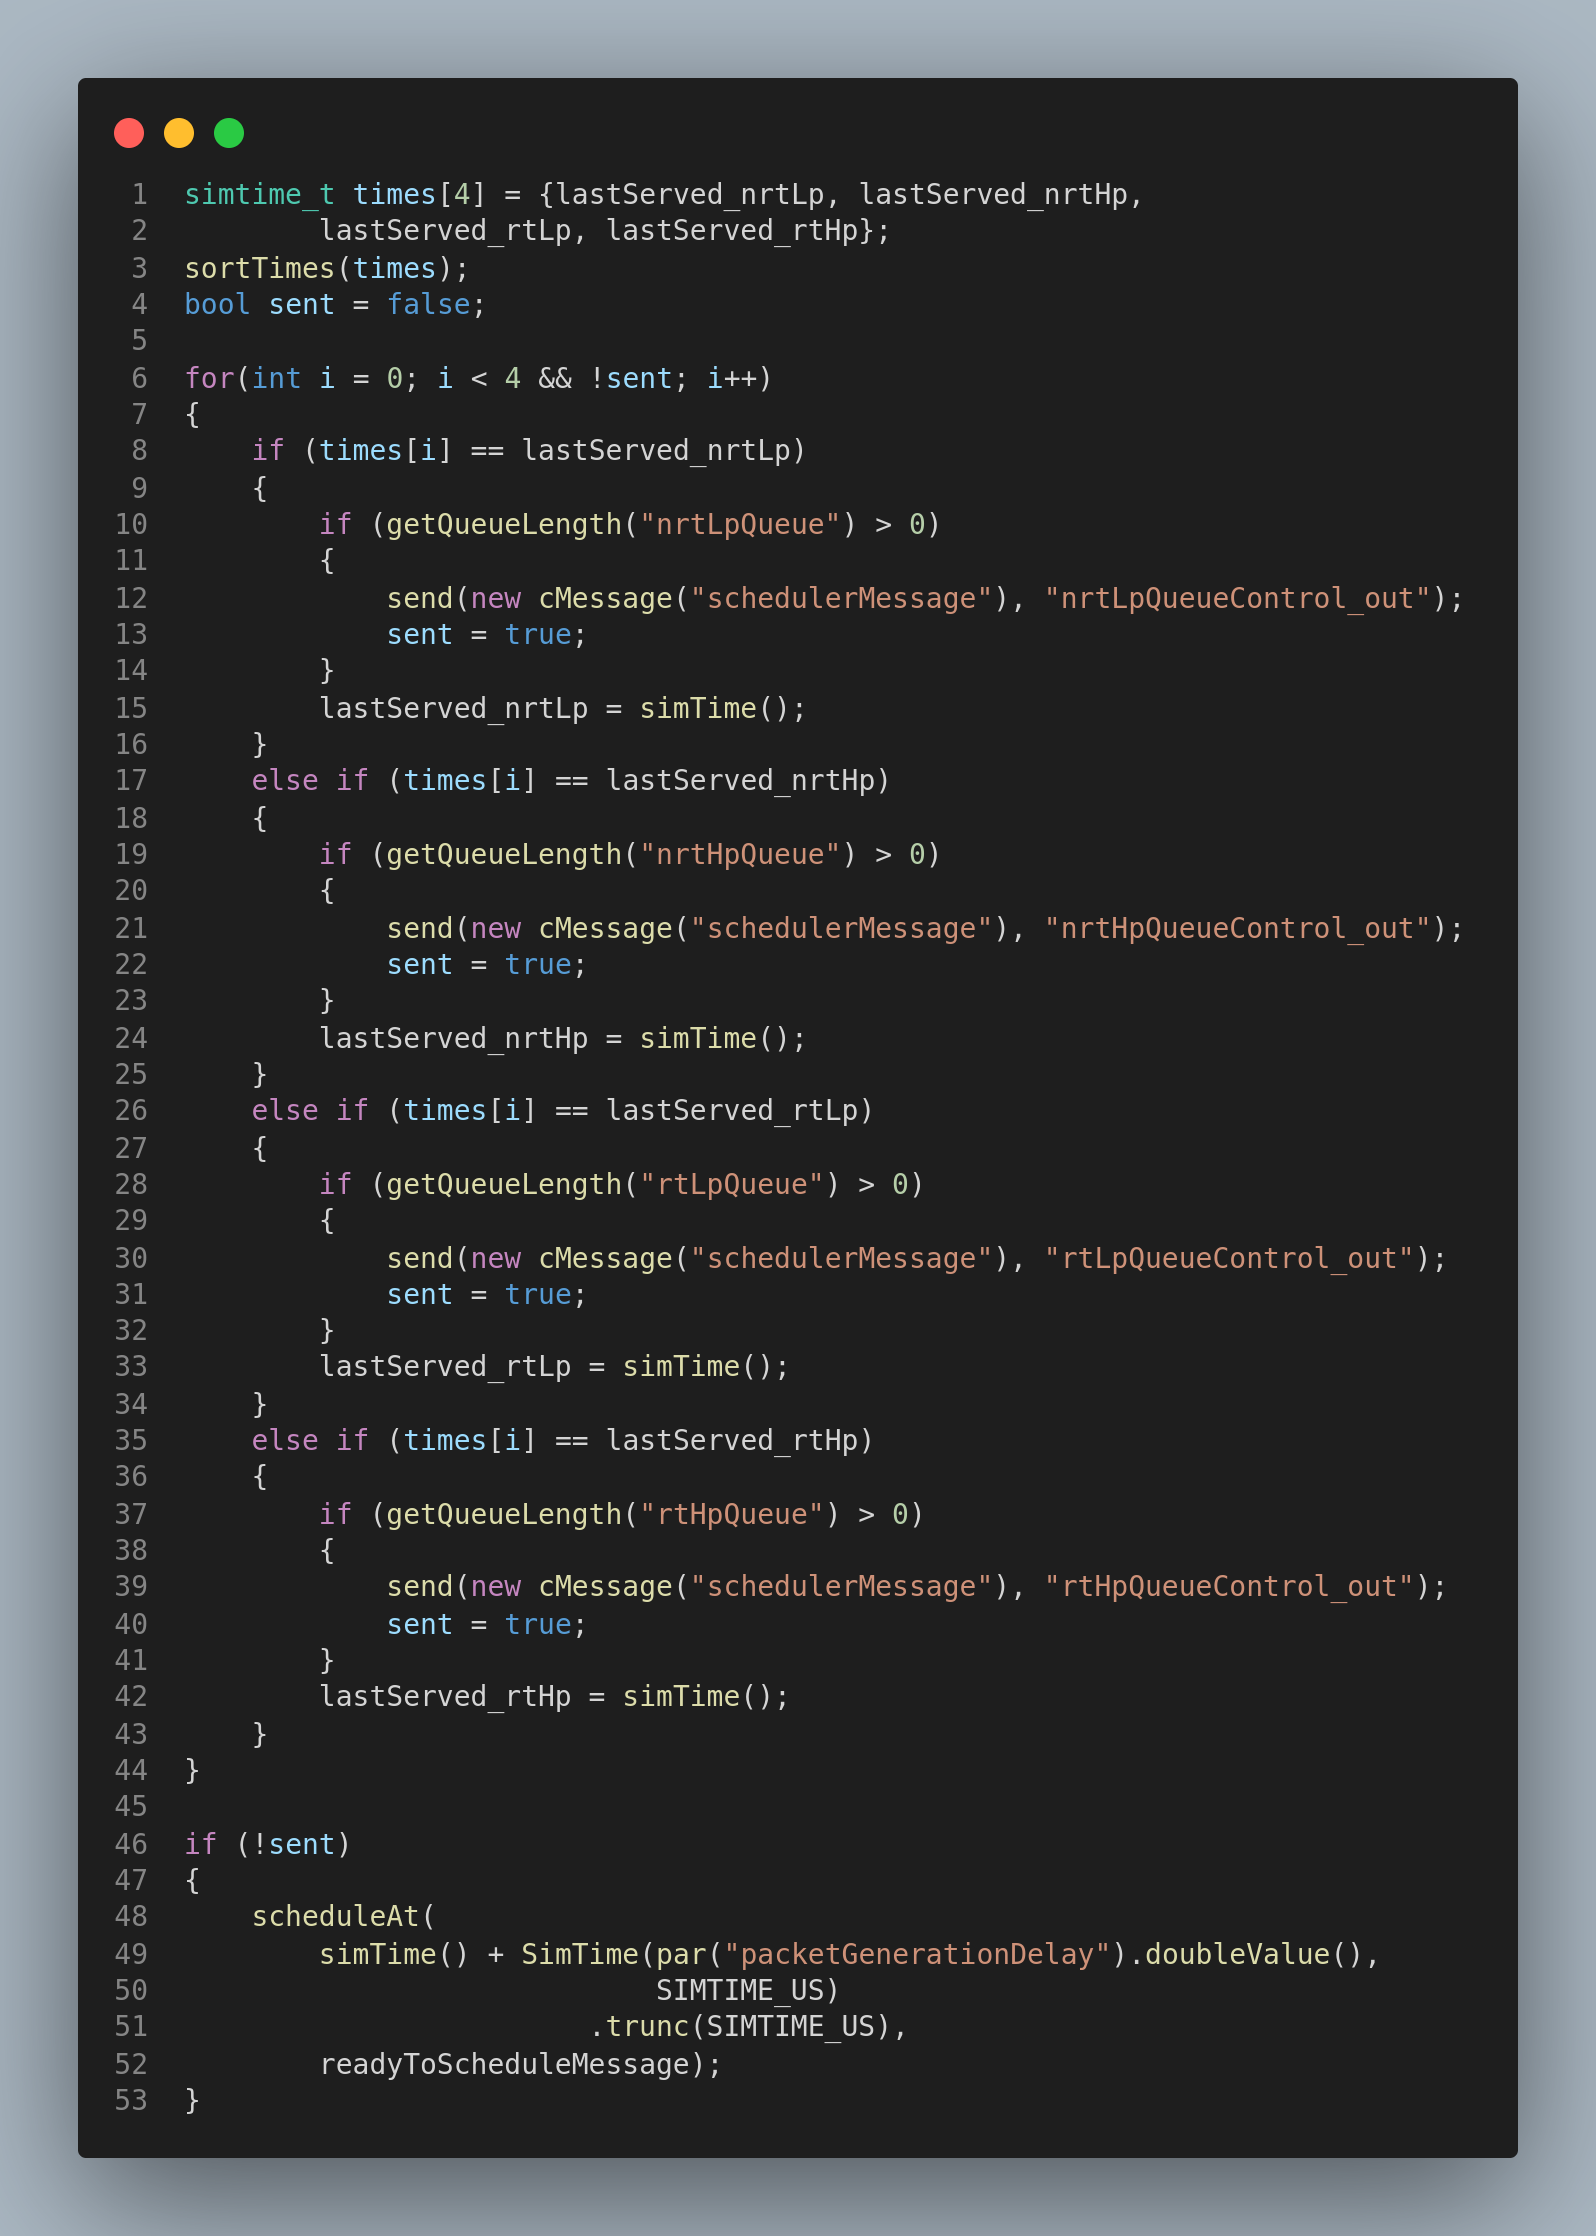
\includegraphics[width=0.74\textwidth]{images/rr_code.png}
            \caption{The inner workings of the Round Robin scheduler}
        \end{figure}
        \pagebreak
        The Round Robin algorithm might look more complex that the previous one, but the underlying principle is in actuality quite simple: the queues which sent a packet recently don't send a packet in the current scheduling cycle, and only the one which sent a packet the longest time ago, sends a packet in the current cycle.
        
        To achieve this, we keep track of the last time at which each queue sent the last packet. When a queue sends a packet, this time is updated to the current simulation time.

        The scheduling algorithm computes the minimum of the mentioned times (the earliest time corresponds to the minimum time), and then checks which queue corresponds to this minimum time. After selecting the queue, the algorithm also checks the length of that queue, so we don't pop from an empty queue, and get an error. As stated before, after each queue sends a packet, its corresponding last-sent-time is updated.

        \subsection{Weighted Round Robin Scheduler}

        The Weighted Round Robin is the most complex of the three presented in this project, but is also the most effective in scheduling the packets to ensure efficiency and speed.

        This algorithm required each class of users to have associated a weight, which will tip the balance in favour of the higher priority users, which will be served more often than the lower priority ones.

        The users' weights are multiplied with the time elapsed since the corresponding queue sent a packet, and the resulting weighted-time is the criterion by which the sender queue is chosen.

        For example, let us consider two priority classes, \textit{low priority} and \textit{high priority}. If the low-priority queue sent a packet 1ms ago, and the high-priority queue sent a packet 500ns ago, with a classic Round Robin algorithm, the low-priority queue should send a packet. With the weights introduced, the 1ms and 500ns times are multiplied with the weights, say 1 for the low-priority queue, and 4 for the high-priority queue. Therefore, the weighted times, which are the basis on which the scheduler decides which queue sends the next packet, are 1ms for the low-priority queue, and 2ms for the high-priority one. Therefore, to the scheduler, it "appears" as if the high-priority queue is the one which sent a packet a long while ago, and the low-priority queue is the one which sent a packet more recently, and so the high-priority queue sends a packet in the current cycle.

        With the weights introduced as described, the queue in priority class $i$ sends packets $\cfrac{w_i}{w_j}$ times as often as the queue in priority class $j$, where $w_i$ and $w_j$ are queue $i$'s weight and $j$'s, respectively.
        \pagebreak

        \begin{figure}[htbp!]
            \centering
            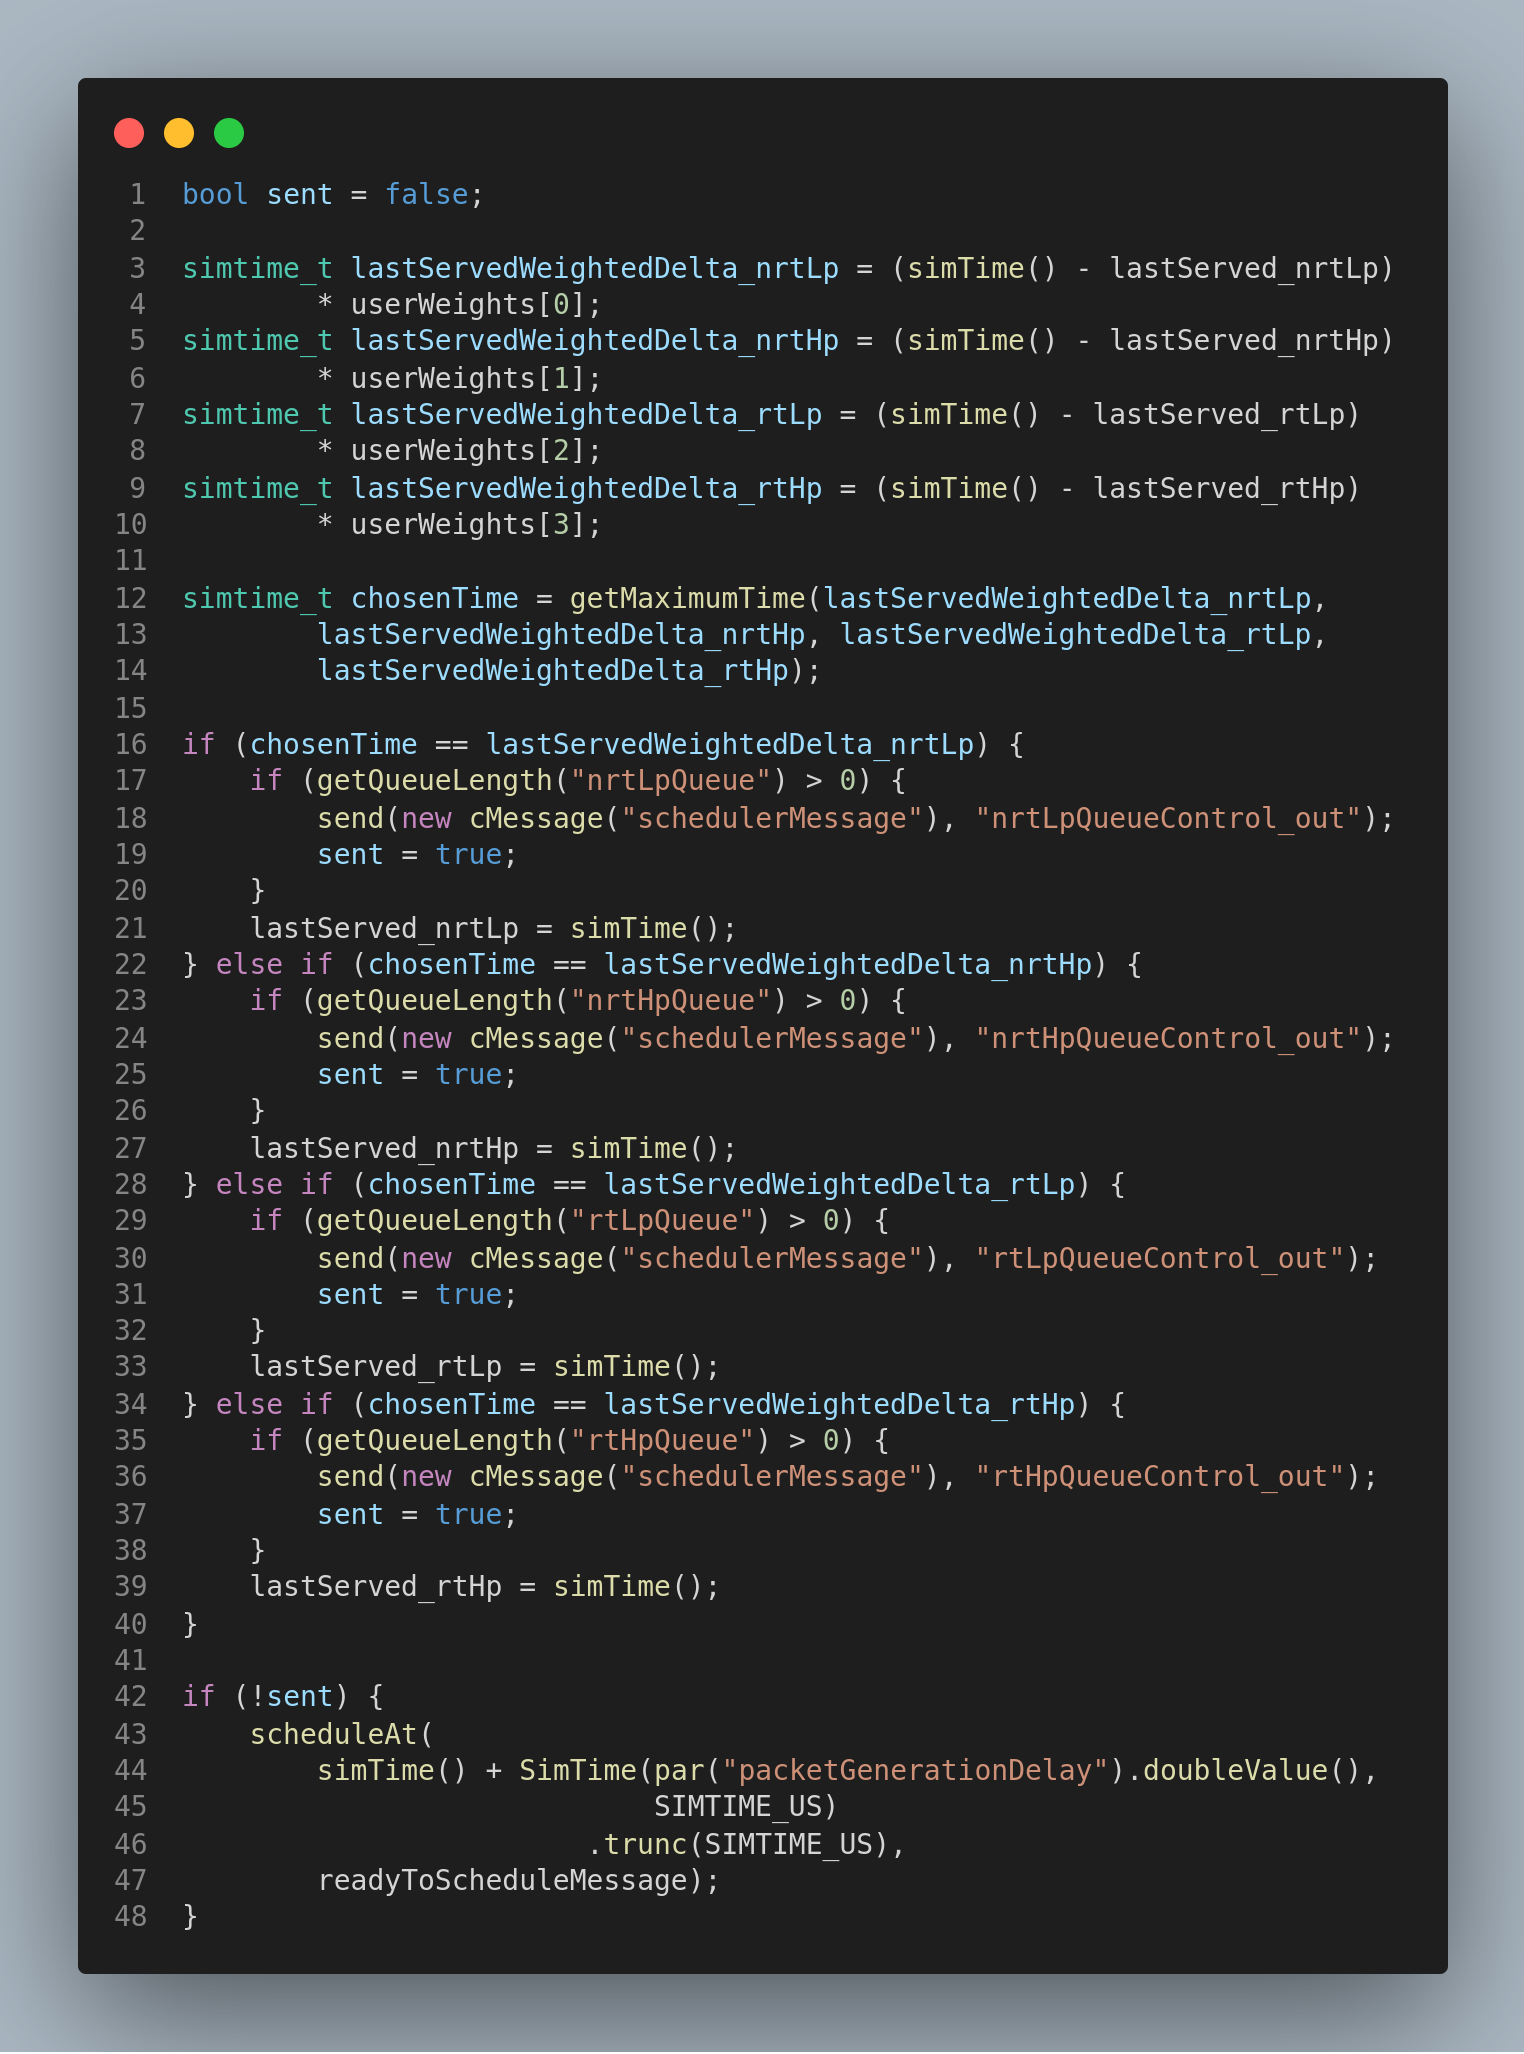
\includegraphics[width=0.74\textwidth]{images/wrr_code.png}
            \caption{The inner workings of the Weighted Round Robin scheduler}
        \end{figure}

    \section{Comparative analysis}
    The following comparative analysis covers all three scheduling algorithms, namely Priority Queueing, Round Robin, and Weighted Round Robin. The system configuration at the time of the benchmarks is:
    \begin{itemize}
        \item{\textbf{50} nrtLp Users, \textbf{40} nrtHp Users, \textbf{30} rtLp Users, and \textbf{20} rtHp Users}
    \item{for the WRR algorithm, the \textbf{weights} are \textbf{1}, \textbf{2}, \textbf{4}, and \textbf{8}, for nrtLp, nrtHp, rtLp, and rtHp respectively}
        \item{the \textbf{IP packet size} varies uniformly between \textbf{100} and \textbf{1500 bytes}}
        \item{the scheduler sends packets to the sink with a \textbf{datarate} of \textbf{1Gbps}}
        \item{the \textbf{packet generation delay} varies triangularly between \textbf{900us} and \textbf{1100us}, with a peak at \textbf{1000us}, corresponding to an average upload rate per user of about \textbf{750KBps}}
    \end{itemize}

        \subsection{Queue Lengths}
        \begin{figure}[htbp!]
            \centering
            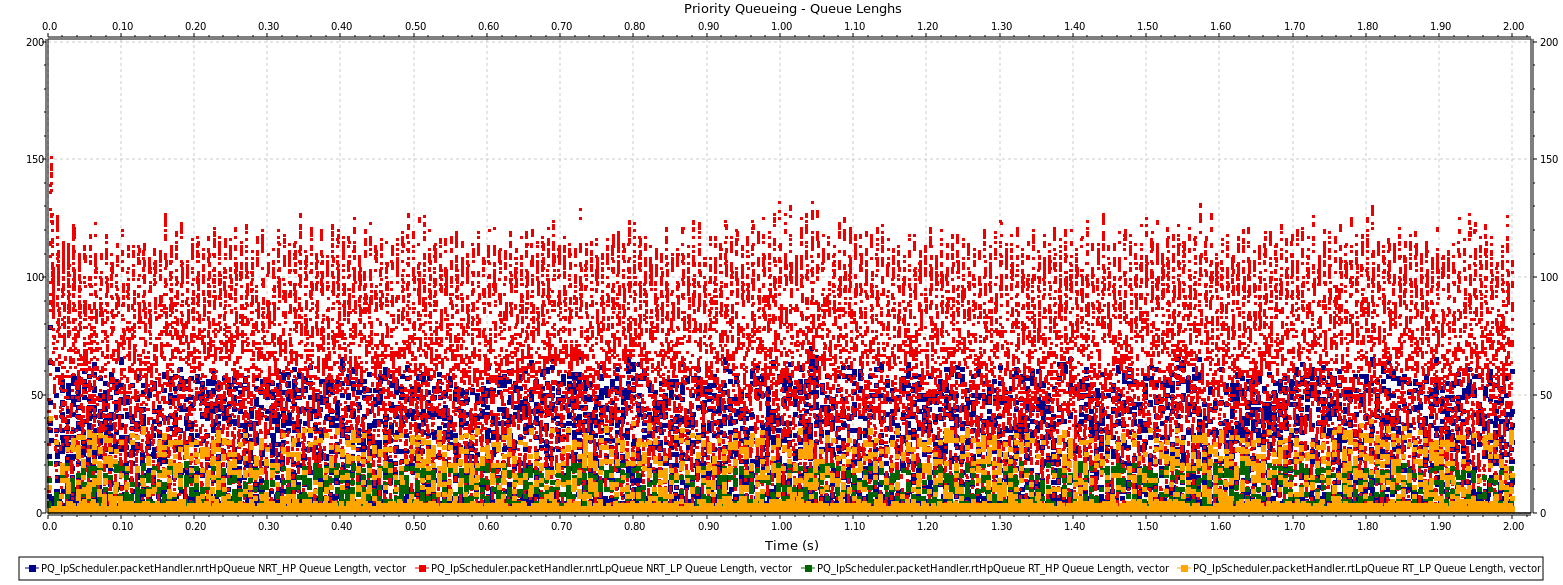
\includegraphics[width=\textwidth]{images/PriorityQueueing_qule.png}
        \end{figure}
        \begin{figure}[htbp!]
            \centering
            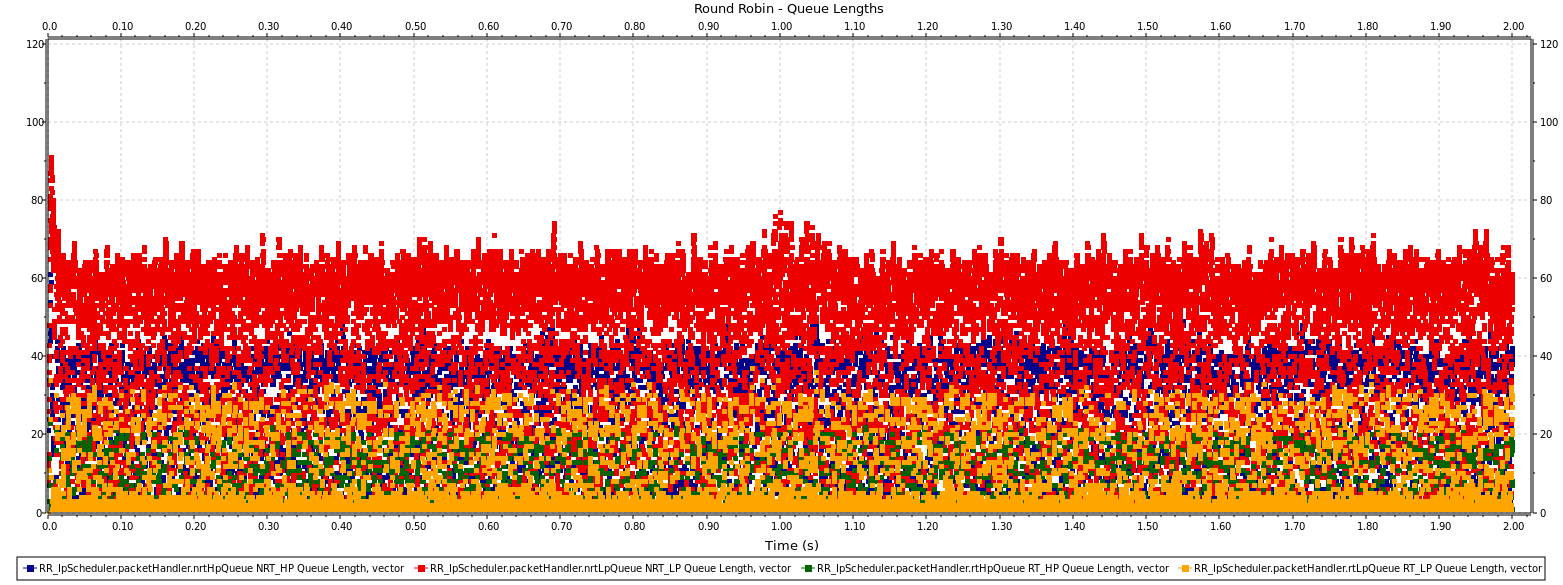
\includegraphics[width=\textwidth]{images/RoundRobin_qule.png}
        \end{figure}
        \begin{figure}[htbp!]
            \centering
            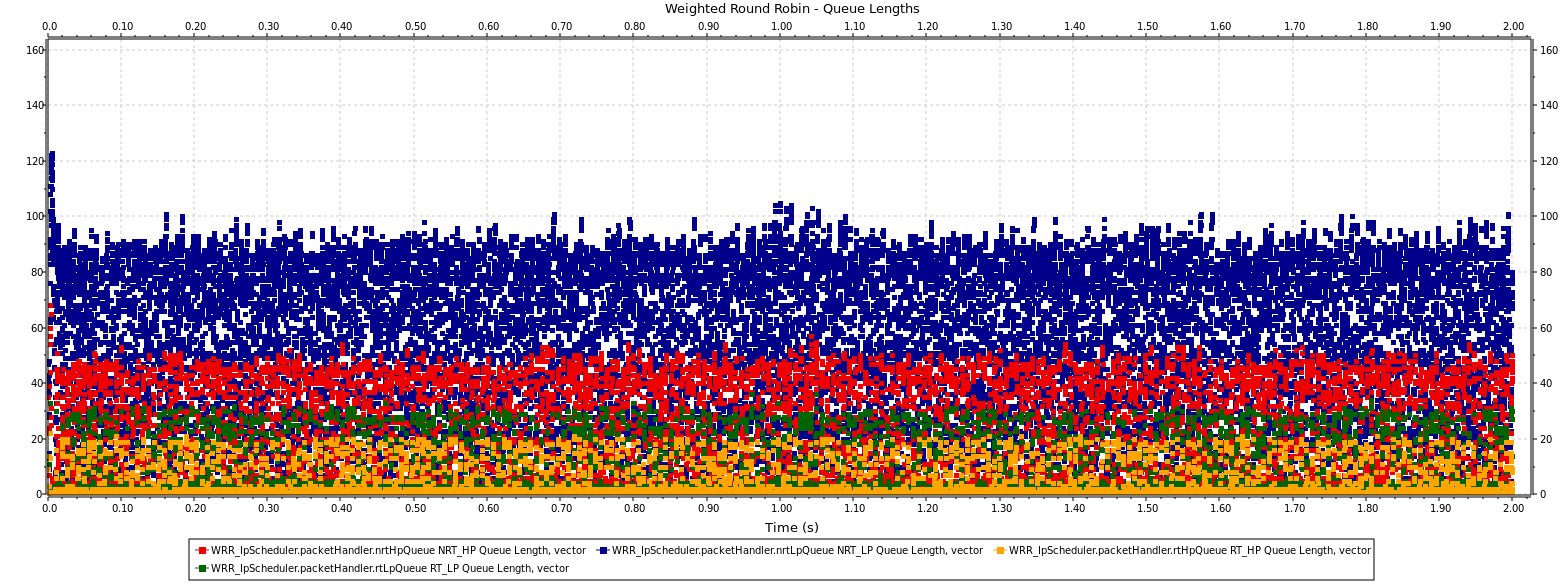
\includegraphics[width=\textwidth]{images/WeightedRoundRobin_qule.png}
        \end{figure}
        \pagebreak
        As we can see in the graphs above, the queue lengths form a nice layered structure, with each priority class having its own band of queue lengths. The lower priority users have higher queue lengths, and the higher priority ones, lower queue lengths.
        
        Below, you can find a table with the mean queue lengths for the four classes of users:
        \begin{table}[htbp!]
            \centering
            \begin{tabular}{l|l|l|l|l|}
                \cline{2-5}
                                                        & nrtLp          & nrtHp          & rtLp          & rtHp          \\ \hline
                \multicolumn{1}{|l|}{Priority Queueing}    & 59.56          & \textbf{10.77} & \textbf{4.46} & \textbf{2.54} \\ \hline
                \multicolumn{1}{|l|}{Round Robin}          & \textbf{44.27} & 19.69          & 8.00          & 4.03          \\ \hline
                \multicolumn{1}{|l|}{Weighted Round Robin} & 54.12          & 14.44          & 5.42          & 2.88          \\ \hline
            \end{tabular}
        \end{table}
        
        The table shows that, when it comes to the queue lengths, the Priority Queueing scheduler is superior, while the Weighted Round Robin scheduler ranks second.

        \subsection{Packet Lifetime}
        \begin{figure}[htbp!]
            \centering
            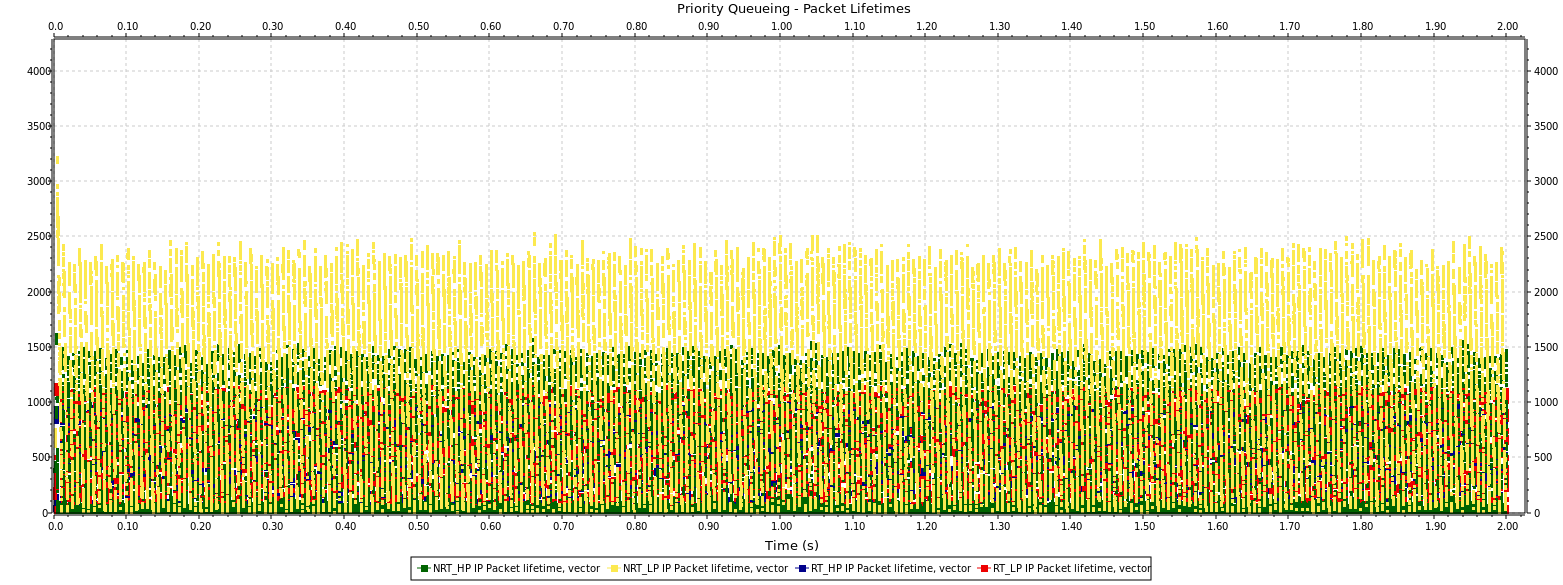
\includegraphics[width=\textwidth]{images/PriorityQueueing_pali.png}
        \end{figure}
        \begin{figure}[htbp!]
            \centering
            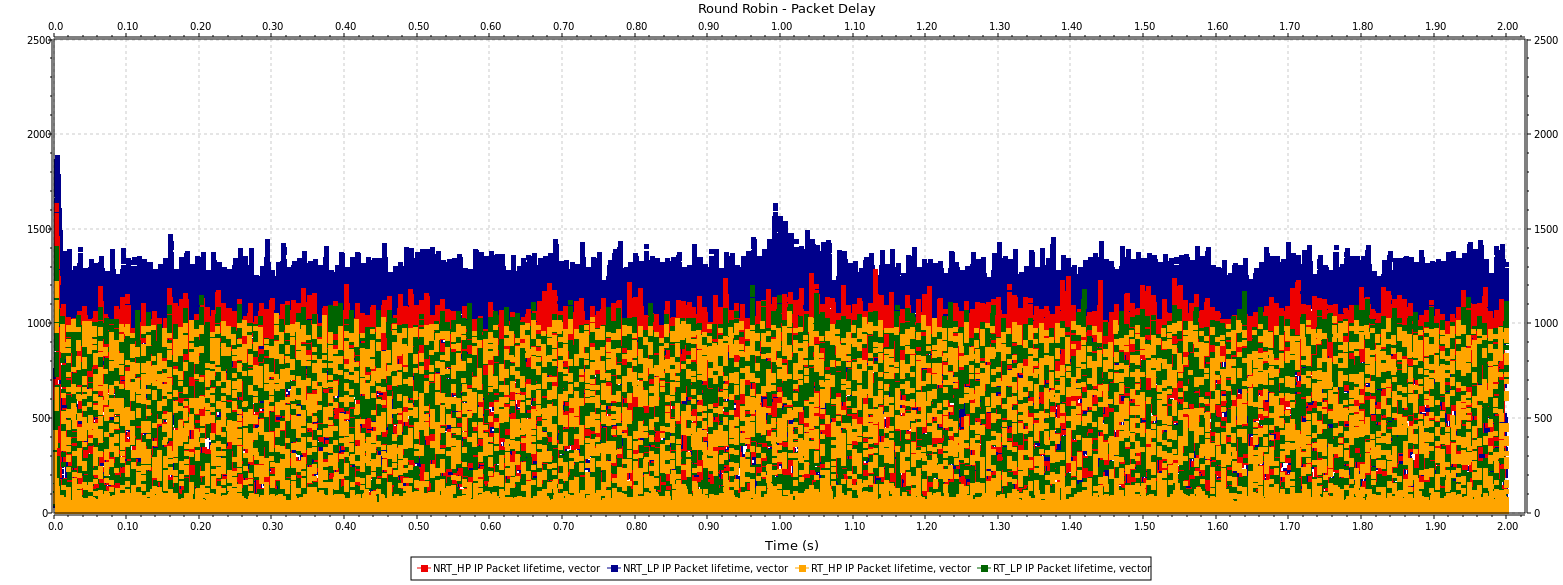
\includegraphics[width=\textwidth]{images/RoundRobin_pali.png}
        \end{figure}
        \pagebreak
        \begin{figure}[htbp!]
            \centering
            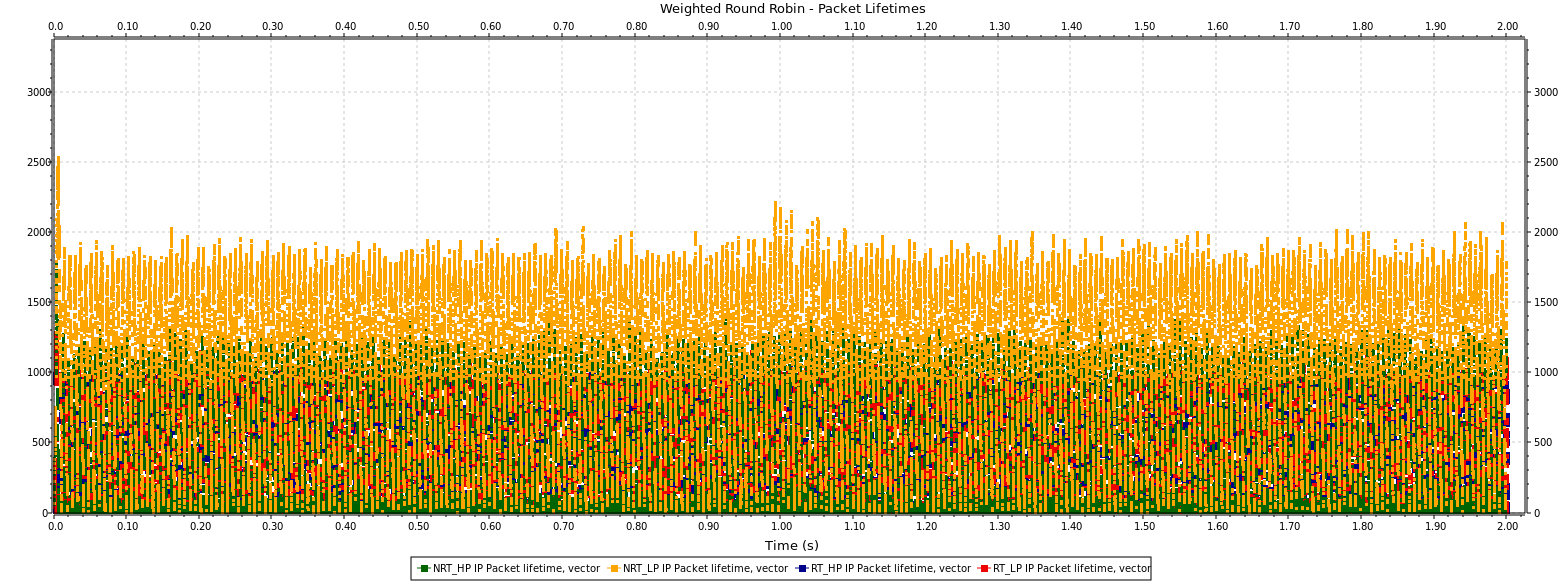
\includegraphics[width=\textwidth]{images/WeightedRoundRobin_pali.png}
        \end{figure}

        The packet lifetime charts also seem to show a layered structure, just like the queue lengths, but this time the layered structured is a little more subtle, the differences being smaller. Also like before, the lower priority users show higher packet delays, while the high priority users show lower delays. It should be noted that the graphs show the packet delay in microseconds.

        Below you can find a table with the mean packet lifetimes for the four classes of users:
        \begin{table}[htbp!]
            \centering
            \begin{tabular}{l|l|l|l|l|}
                \cline{2-5}
                                                        & nrtLp           & nrtHp           & rtLp            & rtHp           \\ \hline
                \multicolumn{1}{|l|}{Priority Queueing}    & 1194.64         & \textbf{254.85} & \textbf{129.31} & \textbf{86.49} \\ \hline
                \multicolumn{1}{|l|}{Round Robin}          & \textbf{884.45} & 476.96          & 264.28          & 161.53         \\ \hline
                \multicolumn{1}{|l|}{Weighted Round Robin} & 1084.30         & 348.13          & 166.12          & 103.02         \\ \hline
                \end{tabular}
        \end{table}

        Again, as before, the Priority Queueing algorithm takes the lead, and the Weighted Round Robin is left in the second place. The Round Robin algorithm seems to favour lower priority users, but falls behind when it comes to the higher priority ones.

    \section{Conclusions}
    As the comparative analysis shows, in the presented case, the Priority Queueing algorithm seems to perform better than its counterparts. The Weighted Round Robin shows the second-best performance, and the Round Robin algorithm, although favouring lower priority users, falls behind in the other categories.

    This, of course, does not match our expectations. We would have expected that the Weighted Round Robin algorithm to come in the first place, the Round Robin to come in second, and the Priority Queueing to be left behind by a long margin. This did not happen, I believe, for a number of reasons:
    \begin{itemize}
        \item{the chosen system configuration (number of users, packet generation rate, etc.) matched a case in which the priority queueing performed better; if we would choose another configuration of parameters, the results would surely change}
        \item{the IP packet generation does not match a real-life scenario; the packets are generated at relatively constant rates, which quite rarely happens in real-life (normally, packets are generated in short bursts of packets, instead of evenly distributed packets)}
        \item{in the case of the Weighted Round Robin algorithm, the weights were chosen on a non-experimental basis; more experiments could reveal a more efficient configuration of weights than the one presented (or, perhaps, the algorithm could be made to make use of adaptive weights, that change according to factors such as network load)}
        \item{I do not exclude the possibility that the other algorithms could suffer improvements, which could tip the balance in one direction or another}
    \end{itemize}
    \pagebreak

    \section{References}
    \begin{enumerate}[label=(\arabic*)]
        \item{\verb|http://staff.cs.upt.ro/~todinca/cad/IP_scheduling.html|}
        \item{\verb|http://staff.cs.upt.ro/~todinca/TPAC/tpac.html|}
        \item{\verb|https://doc.omnetpp.org/omnetpp/manual/|}
        \item{\verb|https://docs.omnetpp.org/tutorials/tictoc/|}
        \item{\verb|https://doc.omnetpp.org/omnetpp/api/|}
    \end{enumerate}
\end{document}